\documentclass[sigconf]{acmart}

\def\BibTeX{{\rm B\kern-.05em{\sc i\kern-.025em b}\kern-.08emT\kern-.1667em\lower.7ex\hbox{E}\kern-.125emX}}
\usepackage{subfigure}

\begin{document}

\title{Approximate Code: A Cost-Effective Erasure Code for Video Applications in Cloud Storage Systems}

\author{Huayi Jin}


%-------------------------ATTANTION-------------------------%
%                                                           %
% red words show the content that requires to be add        %
% blue words need to be perfected or changed                %
%                                                           %
%-----------------------------------------------------------%

\begin{abstract}
Erasure codes are commonly used to ensure data availability in cloud storage systems, where video data produced by autopilot, multimedia industry and security monitoring occupies large amounts of space.
Typical erasure codes, such as Reed-Solomon (RS) \cite{macwilliams1977theory} codes or XOR-based codes use several parity disks to equally back up all data.
However, this is expensive, not only because simultaneous damage of multiple disks is relatively rare, but also due to the ignorance of redundant information inside the data, which results in multiple complete parity disks being excessive.


Therefore, we propose Approximate Codes for video data, which significantly reduce storage overhead and increase availability for more important data segments.
Approximate Codes provide complete recovery when fewer disks fail, and ensure approximate recovery (recover most data) in the event of multiple disk failures.
To demonstrate the effectiveness of Approximate Codes, we conduct several experiments in Hadoop and Alibaba Cloud systems.
The results show that compared with the typical high-reliability erasure code schemes, Approximate Codes reduce the storage overhead by 7.64\% at the expense of reasonable probability of video quality loss.
\end{abstract}

%
% The code below is generated by the tool at http://dl.acm.org/ccs.cfm.
% Please copy and paste the code instead of the example below.
%
\keywords{Erasure Codes, Approximate Storage, Multimedia, Cloud Storage}

\maketitle

\section{Introduction}
Currently, many cloud storage systems use erasure codes to tolerate disk failures and ensure data availability, such as Windows [], Amazon AWS [] or Alibaba Cloud. It is known that erasure codes provide much lower storage overhead and write bandwidth than replication with the same fault tolerance.

Typical erasure codes schemes can be divided into two categories such as RS-based code (RS, LRC), or XOR-based code (...). Other erasure codes (SD, STAIR) use the parity blocks to tolerate sector failures in addition to disk-level fault tolerance.

Video data consumes massive space in cloud storage systems, and this trend is exacerbated as applications demand increased resolution and frame rates. Using multiple copies to ensure video data security will generate storage cost that are several times larger than the original data, which is obviously too expensive, while erasure codes can significantly reduce this cost.

Existing erasure codes are designed to completely recover corrupted data. Typical configurations use triple disk failure tolerant arrays (3DFTS), such as Windows Azure [], which requires at least 3 parity disks. These methods are often excessive because scenes with 3 disks being corrupted at the same time are very rare as well as they do not consider that plenty of video applications can tolerate a certain amount of data loss. For example, video data typically records at least 20 frames per second, which makes losing a few frames difficult for a typical user to perceive. In addition, even if the video data suffers a certain amount of loss, the existing AI-based interpolation algorithm and super pixel algorithm can recover most of the damaged data [].

We also find that video data is usually stored after being encoded to save space, while the encoded video data stream is non-uniformly sensitive to data loss, which makes it inappropriate to provide uniform fault tolerance using conventional erasure codes. With the motion compensation mechanism, common video coding algorithms such as H.264 only needs to store the complete content of key frames and a little part of other frames, which makes other frames rely on the key frames for computation while decoding.

Therefore, we propose Approximate Codes for video data that significantly reduce storage overhead by reducing the parity of data that is not sensitive to errors. In the scenario shown in (Figure 1), the Approximate Codes are designed for systems composed of $n$ disks where $m$ disks are dedicated to coding and another $s$ sectors encoded for the first strip. This allows the data of the first stripe to tolerate any $m+s$ disks corruption, so we specifically store important segments of video data there. With an appropriate data distribution scheme, non-critical data segments will still retain $(n-2m-s)/(n-m)$ data when any $m+s$ disks are corrupted, which makes
recovery schemes such as interpolated or superpixel still effective. The Approximate Codes provide two recovery modes, full recovery and approximate recovery. The former applies to no more than $m$ disk corruptions and recovers all data, the latter applies to no more than $m+$s disks corruptions and retains important data.

\textcolor{red}
{Sixth paragraph:
Contribution of this paper, typically two or three contributions,
(1)	Propose a novel code Approximate Code
(2)	Give some mathematical proof to demonstrate the correctness of Approximate Code
(3)	Conduct several experiments to demonstrate the effectiveness of Approximate Code (no digitals here)}

\begin{table*}[ht]
\centering
\caption{Summary on Various Erasure Codes}
\begin{tabular}{|c|c|c|c|c|c|}
\hline
Name & Fault Tolerance & Storage Overhead & Scalibility & Recovery Cost & \begin{tabular}[c]{@{}c@{}}Computational\\ Complexity\end{tabular} \\ \hline \hline
RS($k,m$) Code & any $m$ disks & $m$ disks & high & high & high \\ \hline
MSR($k,m$) Code & any $m$ disks & $m$ disks & medium & low & very high \\ \hline
Raid 6 & 2 & 2 & low & high & low \\ \hline
SD Code($m,s$) & any $m$ disks and $s$ sectors & $m$ disks and $s$ sectors & low & low & medium \\ \hline
\begin{tabular}[c]{@{}c@{}}Approximate Code($n,m,s,t$)\\ (Important Data)\end{tabular} & any $m+s$ disks & $m$ disks and $s$ sectors & high & high & medium \\ \hline
\begin{tabular}[c]{@{}c@{}}Approximate Code($n,m,s,t$)\\ (Minor Data)\end{tabular} & any $m$ disks & $m$ disks and $s$ sectors & high & high & high \\ \hline
\end{tabular}
\end{table*}

\textcolor{red}
{Seventh paragraph:
organization of the paper}

\section{Related Work and Our Motivation}
Video data can be classified into hot data and cold data, the former requiring high availability and reliability, which often relies on expensive replication approach. The latter's storage usually uses erasure codes schemes, because cold data far exceeds hot data, and erasure codes can guarantee its reliability with low monetary overhead. However, existing erasure code schemes do not consider the characteristics of video data and are not specifically designed for them.

Videos are typically stored in lossy compression, so they are subject to a certain quality loss when stored compared to the original version, and the extent of this quality loss can be specified by the application. For high-quality coded video, it is difficult for the human eye to distinguish the difference between them and the original video, because they preserve most of the brightness information, which human eye is very sensitive to, and some color information is discarded, which human eye is not sensitive to. Therefore, the encoded video data has an uneven degree of importance, that is, the loss of some less important data is tolerable because it's hard for human eyes to detect. On the other hand, loss of important data will have more serious consequences.

This section then introduces the relevant background and our motivation.

\subsection{Existing Erasure Codes}

\textcolor{red}{Here we give some introduction to existing erasure codes
Specifically, we need to illustrate the existing erasure codes for video applications in detail.
Summarize the existing erasure codes in a table (assume Table 1), and illustrate them whether they satisfy the previous requirements in Section II.A}

\subsection{Video Storage}\label{video storage}
For normal HD (resolution 1280$\times$720, 8-bit, 30 fps) video, the amount of raw video data in 1 minute is 4.63 GB, so video data is usually encoded and compressed before storage. Lossy compression is a common method that provides a much lower compression ratio than lossless compression while ensuring tolerable loss of video quality, so we focus on such algorithms.

\begin{figure}[ht]
\centering
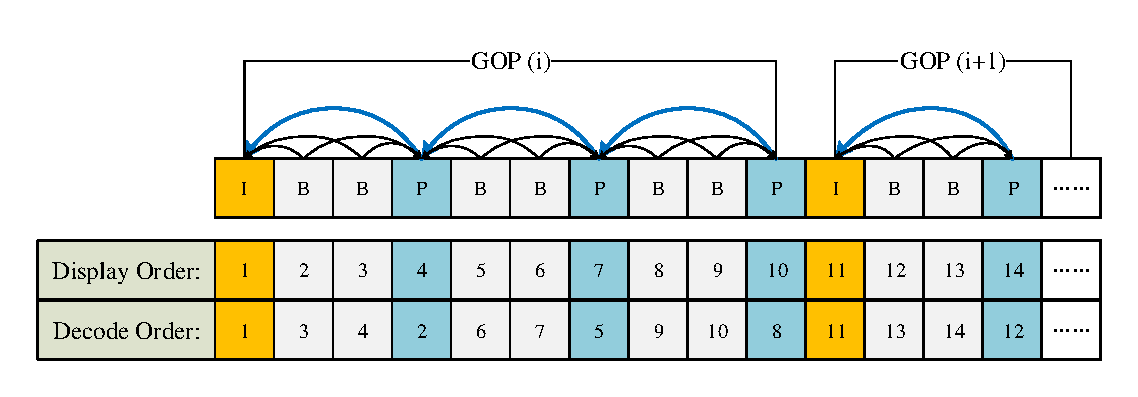
\includegraphics[width=0.45\textwidth]{photo/H264_IPB.pdf}
\caption{A sample of GOPs in H.264}
\label{H264-IPB}
\end{figure}

H.264 is one of the advanced algorithms for this type of work. This coding technique is widely used on platforms such as YouTube because it has higher compression ratio and lower complexity than its predecessor. For the HD video mentioned earlier, H.264 can reduce its size by about 10 times, only 443.27MB.

\textcolor{red}{Something about H.264\dots}

\subsection{Approximate Storage}
Approximate Storage is another way outside of traditional methods of trading off the limited resource budget with the costly reliability requirements, which recently receives more attentions since data centers are faced with storage pressure from the ever-increasing data.

It loosens the requirement of storage reliability by allowing some quality loss of specific data. Therefore, programmers can specify the importance of the data segments and assign them to different storage blocks. The critical data is still safe because they are stored and redundantly backed up by expensive and highly reliable storage devices. Meanwhile, non-critical data is exposed to error, thus increasing storage density and saving cost.

However, it is too naive to store data in approximate storage units indiscriminately. Related research \cite{guo2016high} shows that this can lead to unacceptable data pollution. To ensure data quality in this case, higher error correction costs are required resulting in an increase in overall storage costs.

In the storage of video data, as described in \ref{video storage}, the I frame is the key to decoding the entire GOP. An error in the I frame will cause a decoding error in the P frames and the B frames, and the data loss of the I frame will cause the entire GOP to be undecodable. In contrast, the error or loss of a P frame has less impact, while the B frame is most tolerant of errors because no other frame depends on it.

\textcolor{red}{We define I frames are our important data}

\subsection{Video Frame Recovery: Frame Interpolation}
\textcolor{red}{Add something related to the former subsection}

\textcolor{blue}{In the circumstance of video approximate storage, it's common to lose some minor data making the video incomplete...}

In the circumstance of data loss, it's common to lose some frames and then the video is not complete. One easy way to solve this problem is to store consecutive frames in different disks, so the video is still good for displaying only with fewer frame rates. Another alternative is that we can actually recover the lost frames by applying the a technique named video frame interpolation.

Video frame interpolation is one of the basic video processing techniques, an attempt to synthetically produce one or more intermediate video frames from existing ones, the simple case being the interpolation of one frame given two consecutive video frames. This is a technique that can model natural motion within a video, and generate frames according to this modelling. Artificially increasing the frame-rate of videos enables the possibility of frame recovery. Optical flow is commonly addressed in the video frame interpolation problem. Optical flow is the pattern of apparent motion of objects, surfaces, and edges in a visual scene caused by the relative motion between an observer and a scene. Video frame interpolation algorithms typically estimate optical flow or its variations and use them to warp and blend original frames to produce interpolation results.

Recently, phase-based methods have shown promising results in applications such as motion and view extrapolation \cite{didyk2013joint}\cite{wadhwa2013phase}\cite{meyer2015phase}. These methods rely on the assumption that small motions can be encoded in the phase shift of an individual pixel¡¯s color. Meanwhile, deep learning approaches, and in particular Convolutional Neural Networks (CNNs), have set up new state-of-the-art results across many computer vision problems which also makes big improvements to frame interpolation. In neural networks, optical flow features are trained in a supervised setup mapping two frames to their ground truth optical flow field\cite{dosovitskiy2015flownet}\cite{ilg2017flownet}. Among them, a multi-scale network\cite{van2017frame} based on recent advances in spatial transformers and composite perceptual losses as well as a context-aware Synthesis approach\cite{niklaus2018context} have so far produced the best results in terms of PSNR and middlebury benchmark respectively.

\textcolor{blue}{All the frame interpolation method are based on that we have the input of full images of two consecutive frames (maybe one or two missing in the middle). However, in the popular coding format like H.264, only I frame have full image data of itself, and all the other image data is dependent on that in I frames. Without an I frame, the following ones that depend on it will go invalid and be impossible for recovery which means I frames require more storage overhead to ensure its integrity and reliability.}

\subsection{Our Motivation}
Based on Table [], the existing erasure codes cannot meet the requirements of video applications in the cloud storage system due to the following reasons. First, existing erasure codes generally reach or exceed 3DFTS, and use more than 3 parity disks. However, the simultaneous damage of 3 disks is very rare, and the storage overhead paid for this is too large. Second, the existing erasure codes provide the same fault tolerance for all data without distinction, which results in the same reliability of important data that is sensitive to errors and data that is robust. To solve these two problems, we propose a new erasure code called approximation code. It provides different fault tolerance for important and non-critical data to reduce storage overhead and protect critical data better.

\section{Approximate Code}
In this section, we introduce the design of Approximate Code and its properties through a few simple examples. For convenience of description and without loss of generalizability, we use fewer data blocks (resulting in greater storage overhead). A more optimized parameter selection scheme for practical applications will be introduced in \ref{evaluation}.

\subsection{Design of Approximate Code}
In a system of $n$ disks, each disk can be divided into multiple sectors. We focus on the $r$ sectors of the same logical position of each device, and we treat these $r$ sectors as a \emph{chunk}. The $r \times n$ sectors of $n$ chunks constitute a stripe, as shown in Figure \ref{chunk-sector} . We also use the term symbol in coding theory to refer to sectors. Since each strip is independent of the entire system, we only consider a single strip.

\begin{figure}[ht]
\centering
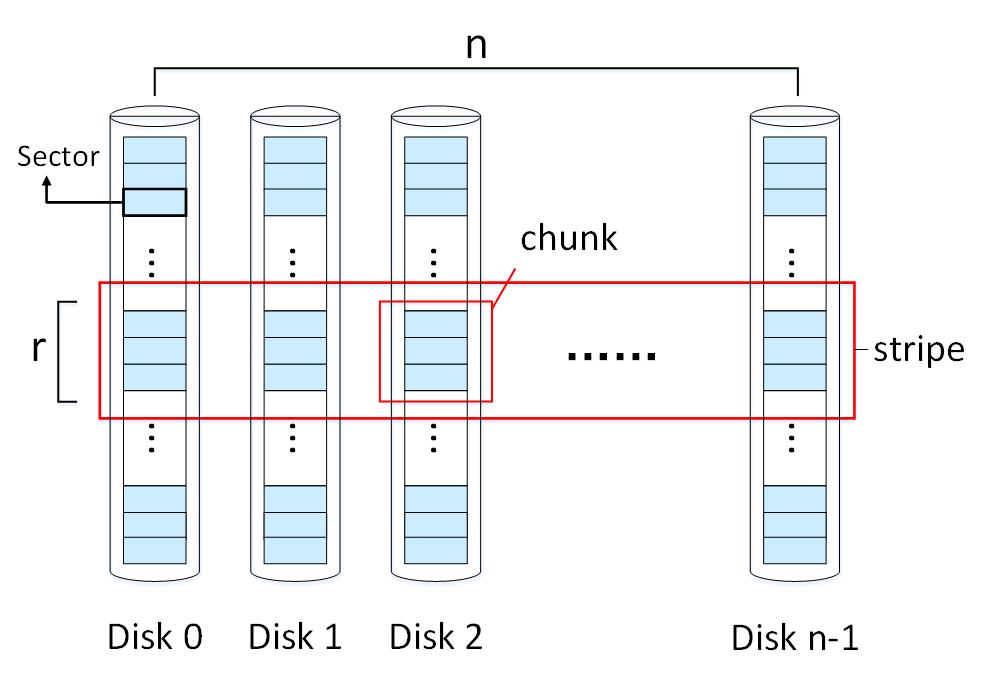
\includegraphics[width=0.35\textwidth,height=40mm]{photo/chunk-sector.JPG}
\caption{A sample of chunks and sectors}
\label{chunk-sector}
\end{figure}

In the $n$ chunks of each stripe, $m$ ones are for coding and in the remaining $n-m$ chunks. 
We use $s \times t$ additional sectors for coding important data, where $s$ is the number of the columns and $t$ is the number of the rows, as shown in Figure \ref{apcode-72522}.
For convenience, we label $h=n-m-s$ as the number of columns of important data that is storaged in $h \times t$ blocks in our assumption.

\textcolor{blue}{Although the choice of parameter $r$ is arbitrary, we recommend setting it to $r=s+h$ and the relevant instructions will be shown in ...}

Based on the above definition, our design has 4 configurable parameters $(n, m, r, s,t)$ that uniquely determine the construction of Approximate Code.
Figure \ref{apcode-72522} shows an example of Approximate Codes with $n = 7$, $m = 2$, $r=5$, $s=2$ and $t = 2$, where we label the data disks with $d_{i,j}$, the important data parity sectors with $q_{i,j}$ and the minor parity sectors with $p_{i,j}$.

We then define the set of sectors as follows:
\begin{itemize}
    \item $D_I=\{d_{i,j}|0\leqslant i < t, 0\leqslant j < h \}$ important data sector set.
    \item $D_M=\{d_{i,j}|t\leqslant i < r, 0\leqslant j < n-m \}$ minor data sector set.
    \item $Q=\{q_{i,j}|0\leqslant i < t, 0\leqslant j < s \}$ important parity sector set. 
    \item $G=\{p_{i,j}|0\leqslant i < r, 0\leqslant j < m \}$ global parity sector set.
\end{itemize}

\begin{figure}[h]
\centering
\subfigure[sector label and encoding process]{
    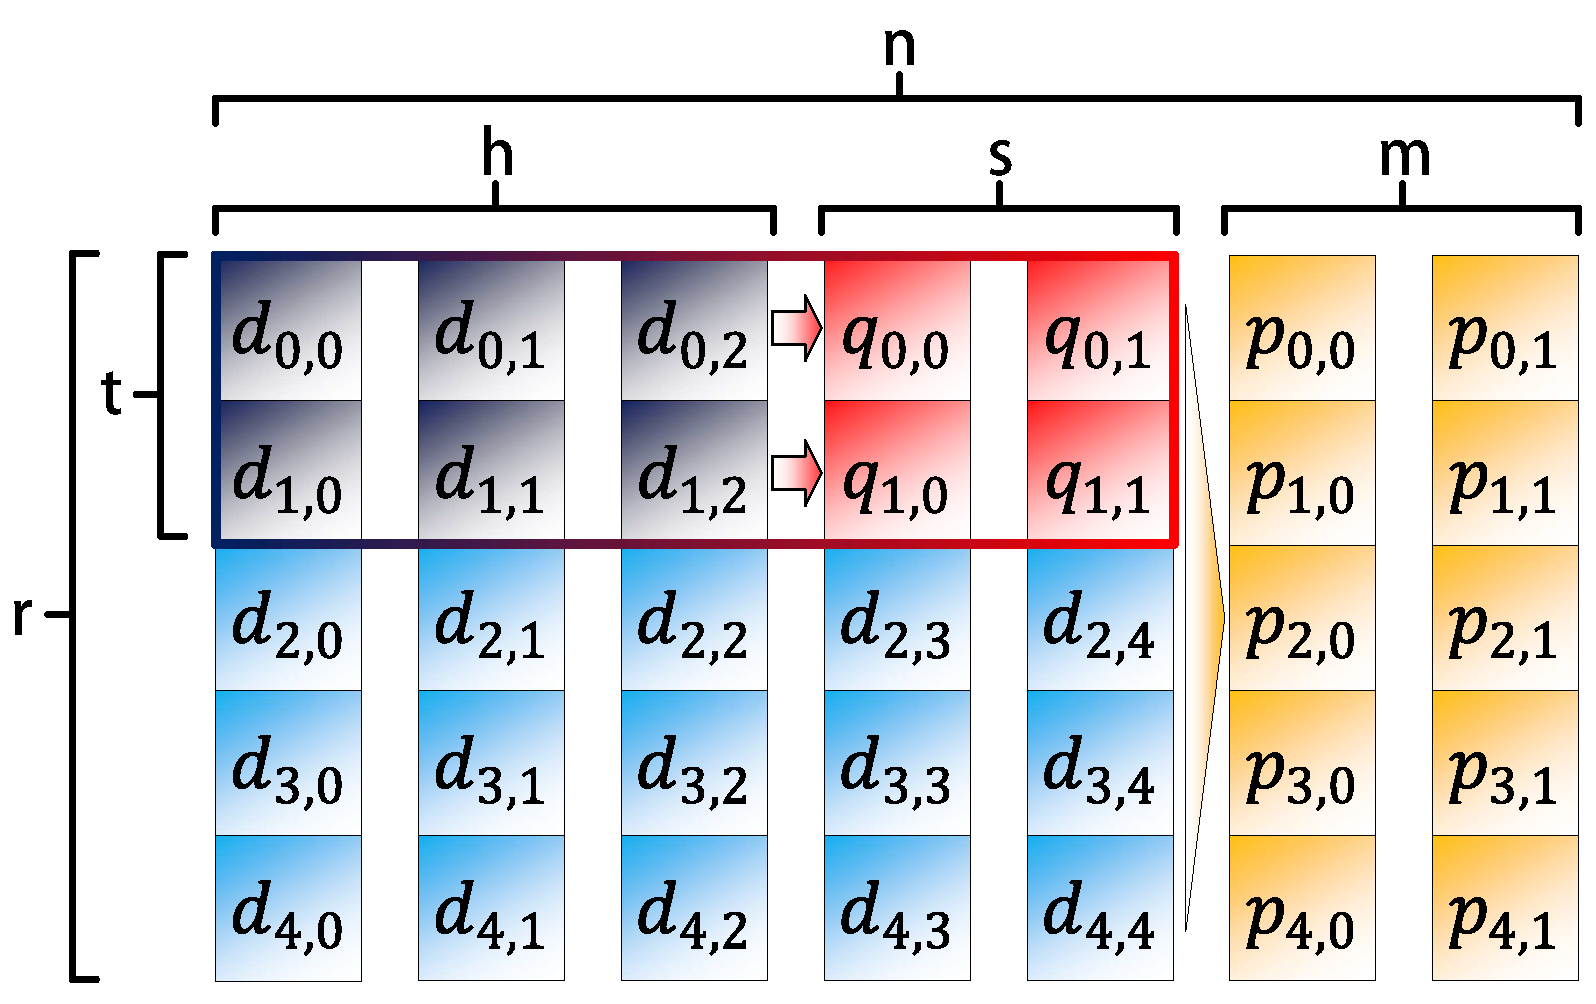
\includegraphics[width=0.32\textwidth]{photo/apcode-72522.PDF}
    \label{apcode-72522-a}
}
\subfigure[sector sets]{
    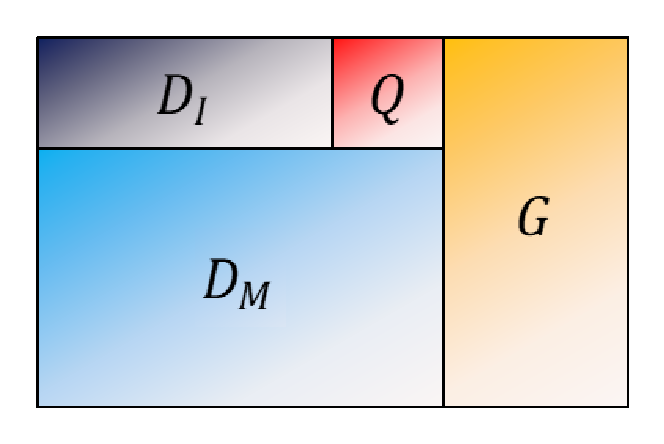
\includegraphics[width=0.13\textwidth]{photo/DDQG.PDF}
    \label{apcode-72522-b}
}
\caption{A sample of Approximate Codes $(7,2,5,2,2)$ with 7 chunks where 2 of them are parity chunks (orange set $G$) and each chunk has 5 sectors. In this example, there are 6 sectors (dark blue set $D_I$) for important data, 15 sectors (light blue set $D_M$) for minor data and 4 other sectors (red set $Q$) are designed for encoding important data.}
\label{apcode-72522}
\end{figure}

\subsection{Encoding and Decoding Process}
In this section, we use Figure \ref{apcode-72522} to illustrate the encoding and decoding process of Approximate Code$(7,2,5,2,2)$.

The encoding process consists of two phases: the important coding phase (\emph{I-Phase}) and the global coding phase (\emph{G-Phase}). 
The \emph{I-Phase} is expressed as two red arrows in the blod box, where $Q$ is generated to verify $D_I$, and
the \emph{G-Phase} is expressed as a yellow triangle arrow, where $G$ is generated to verify $D_I$, $D_M$ and $Q$.

The decoding process provides two modes: the approximate recovery mode and the full recovery mode.
When no more than $m$ divices fail, Approximate Code guarantees full recovery of lost data.
When the number of failed devices is larger than $m$ but no more than $m+s$, Approximate Code guarantees full recovery of lost important data, which require $D_I$, $Q$ and part of $G$ for joint recovery.

It should be noted that in the calculation of $G$ in \emph{G-Phase} and in the decoding process in full recovery mode, we consider $D_I$, $D_M$ and $Q$ as the same, and the minimum coding unit is chunk. That is, when we do not distinguish the importance of the data($s,t = 0$), the Approximate Code is a typical $m$ disk redundancy code.

In general, Approximate Code performs extra parities on important data.
Since our design guarantees the important data, the important parity and the minor data blocks completely fill $n-m$ chunks, we can construct the remaining $m$ parity chunks in any way, as long as their parity method are linearly independent of the way the important parity blocks are. Therefore, EC methods such as RS-based, XOR-based, MSR, MDS or PMDS codes can be used to construct Approximate Code because it is essentially a way of data classification and data distribution, and current EC schemes do not assume anything about data feature.

\textcolor{blue}{We then introduce RS-based and XOR-based Approximate Code}
\subsubsection{RS-based Approximate Code}

In \emph{I-Phase}, we use RS(3,2) to encode 3 groups of important data sectors and generate 2 groups of parity sectors labeled with $q_{i,j}$. The calculation of $q_{i,j}$ are defined by equation (\ref{q_ij}), where $\alpha_k$ is the coefficient in Galois Field (GF). The coding coefficient matrix is transformed from the Vandermonde matrix by elementary transformation.

\textcolor{red}{Coding matrix like below?}

\begin{equation}
\begin{pmatrix} 
1&  1&  1\\
\alpha_0 & \alpha_1 & \alpha_2 \\
\alpha_0^2+\alpha_3^2+\alpha_4^2*\alpha_0 & \alpha_1^2 +\alpha_3^2+\alpha_4^2*\alpha_1 & \alpha_2^2+\alpha_3^2+\alpha_4^2*\alpha_2  \\
\alpha_0^3+\alpha_3^3+\alpha_4^3*\alpha_0 & \alpha_1^3 +\alpha_3^3+\alpha_4^3*\alpha_1 & \alpha_2^3+\alpha_3^3+\alpha_4^3*\alpha_2  \\
\end{pmatrix} 
\end{equation}

For example, $q_{1,1} = \alpha_0 d_{1,0} + \alpha_1 d_{1,1} + \alpha_2 d_{1,2}$.
\begin{equation}\label{q_ij}
    q_{i,j} = \sum_{k=0}^{h-1} \alpha_k^{j} d_{i,k}
\end{equation}

In \emph{I-Phase}, we use RS(5,2) to generate 2 parity chunks labeled with $p_{i,j}$ from 5 chunks consist of data sectors and important parity sectors. The calculation of $p_{i,j}$ are defined by equation (\ref{p_ij_1}) and (\ref{p_ij_2}).
For example, $p_{1,1} = \alpha_0^3 d_{1,0} + \alpha_1^3 d_{1,1} + \alpha_2^3 d_{1,2} + \alpha_3^3 q_{1,0} + \alpha_4^3 q_{1,1}$.

\begin{equation}\label{p_ij_1}
    \mathop{p_{i,j}}\limits_{i<t} = 
    \sum_{k=0}^{h-1} \alpha_k^{s+j} d_{i,k} +
    \sum_{k=0}^{s-1} \alpha_{k+h}^{s+j} q_{i,k}
\end{equation}
\begin{equation}\label{p_ij_2}
    \mathop{p_{i,j}}\limits_{i \geqslant t} = 
    \sum_{k=0}^{n-m-1} \alpha_k^{s+j} d_{i,k}
\end{equation}

The full recovery decoding process of RS-based Approximate Code is obvious since it is the same as the decoding process of RS(5,2).
For the approximate decoding process, there are 4 independent equations that can tolerate any 4 disk failures because the coding coefficient matrix is full rank.

\subsubsection{ XOR-based Approximate Code}
\textcolor{red}{It is difficult to design XOR-based codes that m=2,s=1. Codes like EVENODD or STAR cannot be used to recover the important data when 3 disks fails. However, the desgin of m=1 is easy, because we only use horizontal parity blocks. }

\textcolor{red}{One other way to generate XOR parity sectors is to divide each sector into multiple smaller blocks and apply EVENODD or RAID6 on them. This might be too complex but its correctness is easy to proof.}

\subsection{\textcolor{red}{Proof of Correctness}}

\subsection{Intermediate Layer}\label{Intermediate Layer}
Compared with the traditional scheme that does not consider the meaning of the upper layer data, the Approximate Code pays attention to the difference of the importance of the data, so an intermediate layer between the upper layer application and the underlying distributed storage module is needed to preprocess the data. In our design, the middle layer performs automatic data identification and data distribution, implementing \emph{I-Phase} in the encoding process and approximate recovery mode in the decoding process.

\subsubsection{Data Identification}
For H.264 video data, we define I frames as important data, and P frames and B frames as minor data based on the analysis in the \ref{video storage}. In practical, video data is rarely stored in the original form of H.264 streams (``.264'' files), but is usually storaged in an file such as ``.mp4'' files containing information such as audio. We transcode video files into raw video streams and other data, and we define these non-video data as important because they contain information that the video can't provide and only take up a small amount of space. The feasibility of this definition will be confirmed in \ref{evaluation}.

\subsubsection{Data Distribution}
Fortunately, in an H.264 stream, each GOP begins with an I frame followed by a series of P and B frames. Therefore, we store data in units of GOPs. Our main purpose is to store I frames and other frames separately. For non-video data, we distribute it into multiple GOPs and treat it as a special part of the I frame. In the following description, we no longer consider such data especially and simply refer to them as I-frames.
Our data distribution algorithm is as follows:

\textcolor{red}{Need to draw an algorithm table from the following description}

1. Calculate the important data ratio of each GOP in a stripe, and remember that the highest one is $\omega_{max}$.

2. Adjust $t$ to find the important rate $\omega_{act}$ closest to $\omega_{max}$

3. Divide each GOP into two parts: $\omega_{act}$: $1-\omega_{act}$.

4. Store the former in $D_I$, the latter in $D_M$.

In this regard, the decoding process is as follows:

1. Read the entire strip and find the nmrst parameter of the strip record

2. Calculate $\omega_{act}$ based on parameters

3. Read the $I$ frame from $D_I$ until the next I frame is encountered

4. Calculate the length read in 3, multiply by $(1-\omega_{act})/\omega_{act}$ , and read this length in $D_M$.

5. Combine I frames with other frames.
The data distribution scheme is shown in the figure \ref{Data-distribution-v2}.

\textcolor{blue}{Some description about the figure...}

Our approach can be applied to a variety of other data types. In fact, encoded multimedia data mostly has the property of coexisting important data and non-essential data, such as PTC encoding used in image storage[][].

\begin{figure}[h]
\centering
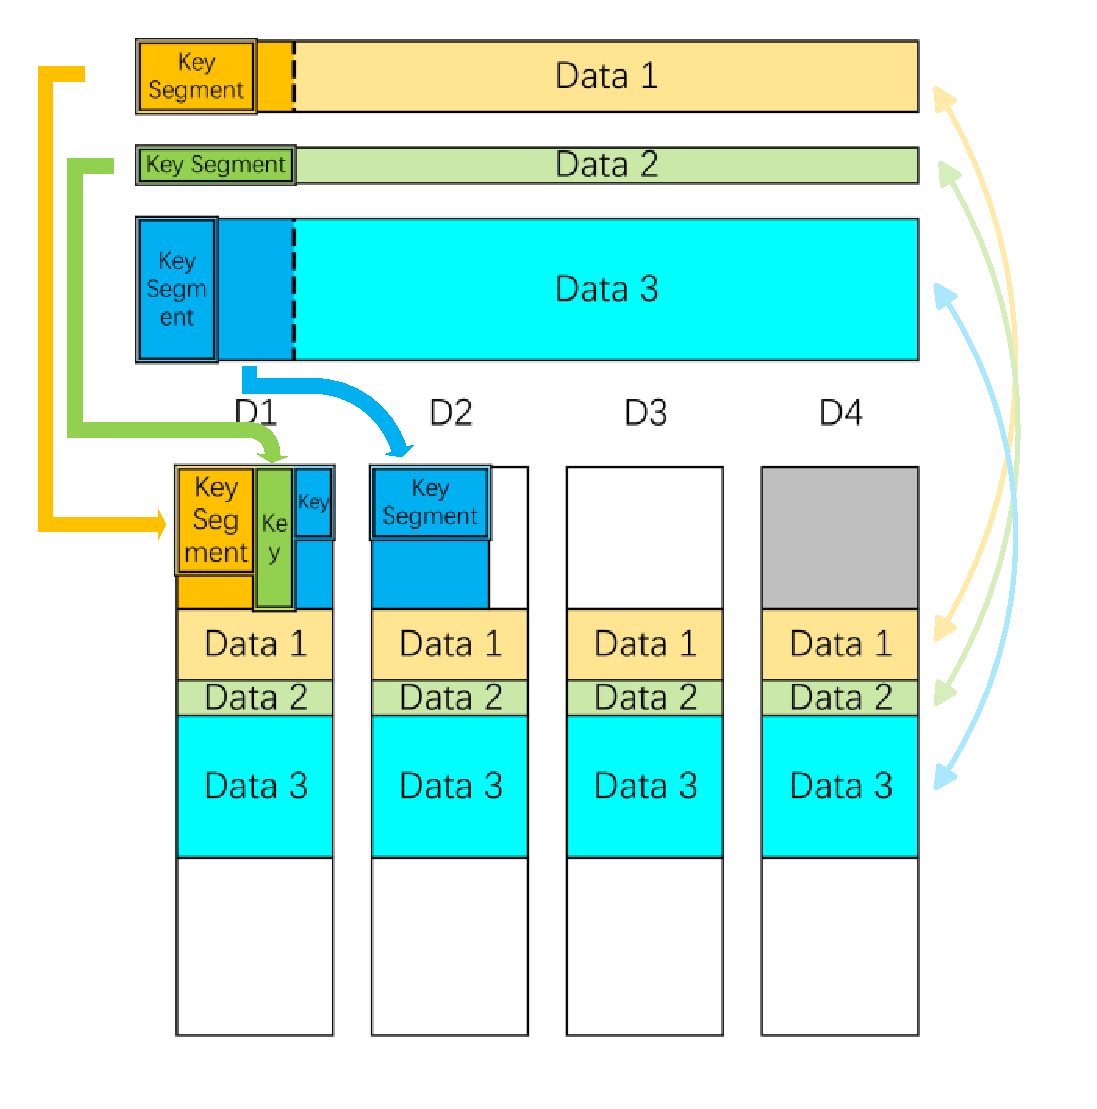
\includegraphics[width=0.35\textwidth]{photo/Data-distribution-v2.PDF}
\caption{1}
\label{Data-distribution-v2}
\end{figure}

\subsection{Properties of Approximate Code}

\section{Evaluation}\label{evaluation}
\begin{table}[ht]
\begin{tabular}{|c|c|c|c|c|}
\hline
\begin{tabular}[c]{@{}c@{}}Code\\ Config\end{tabular} & \begin{tabular}[c]{@{}c@{}}Storage \\ Efficiency\end{tabular} & \begin{tabular}[c]{@{}c@{}}FT\\ (Imp)\end{tabular} & \begin{tabular}[c]{@{}c@{}}FT\\ (Minor)\end{tabular} & \begin{tabular}[c]{@{}c@{}}Important \\ Rate\end{tabular} \\ \hline
(6,2,4,1,2) & 1.600 & 3 & 2 & 0.200 \\ \hline
(8,2,6,1,1) & 1.371 & 3 & 2 & 0.143 \\ \hline
(10,2,8,1,1) & 1.270 & 3 & 2 & 0.111 \\ \hline
(11,2,9,1,1) & 1.238 & 3 & 2 & 0.100 \\ \hline
(11,3,7,1,1) & 1.400 & 4 & 3 & 0.127 \\ \hline
(13,3,10,1,2) & 1.327 & 4 & 3 & 0.184 \\ \hline
(8,2,6,1,2) & 1.412 & 3 & 2 & 0.294 \\ \hline
(8,2,4,1,2) & 1.455 & 3 & 2 & 0.455 \\ \hline
(10,2,6,2,2) & 1.364 & 4 & 2 & 0.273 \\ \hline
(11,3,8,2,2) & 1.467 & 5 & 3 & 0.200 \\ \hline
\end{tabular}
\end{table}
\subsection{An Evaluation methodology}
\subsubsection{Erasure Codes in Our Comparisons}
\subsubsection{Platforms and Configurations}
\subsubsection{Metrics}
\subsubsection{Parameters and Assumption in Our Evaluation}


\subsection{Results}
\subsection{Analysis}
Illustrate why Approximate Code achieve high reliability with low cost
\section{Conclusion}

%
% The acknowledgments section is defined using the "acks" environment (and NOT an unnumbered section). This ensures
% the proper identification of the section in the article metadata, and the consistent spelling of the heading.
\begin{acks}
To Robert, for the bagels and explaining CMYK and color spaces.
\end{acks}

%
% The next two lines define the bibliography style to be used, and the bibliography file.
\bibliographystyle{ACM-Reference-Format}
\bibliography{ApproximateCode}

\end{document}
